% Manuscript for the Journal of Graph Algorithms and Applications, draft 1, 2026-11-05 (log.md 0067).
% Class: jgaa-art.cls from https://jgaa.info/JGAA-LaTeX.zip, read 2026-11-05, unmodified (template.md).
\documentclass{jgaa-art}

\usepackage{graphicx}
\usepackage{amsmath}
\usepackage{amssymb}
\usepackage{array}
\usepackage[mathlines]{lineno}
\graphicspath{{../../figures/pdf/}}

\begin{document}
% --------------------------------------------------------------------
\doi{}
\Issue{0}{0}{0}{0}{0}
% --------------------------------------------------------------------
\HeadingAuthor{Sulaiman et al.}
\HeadingTitle{Sharing Work Within Batches for Exact Dynamic Cycle Counting}
% --------------------------------------------------------------------
\title{Sharing Work Within Update Batches for Exact Dynamic Counting of Triangles, 4-Cycles and 5-Cycles: An Experimental Study}
\Ack{This research received no specific grant from any funding agency in the public, commercial, or not-for-profit sectors.}
% --------------------------------------------------------------------
\authorOrcid[utemim]{Hamzah Asyrani Sulaiman}{asyrani@utem.edu.my}{0000-0002-7714-5967}
\authorOrcid[utemim]{Shafina binti Abd Karim Ishigaki}{shafina@utem.edu.my}{0000-0003-4551-0824}
\authorBOrcid[utemse]{Asniyani Nur Haidar binti Abdullah}{asniyani@utem.edu.my}{0009-0008-5148-2341}
\authorOrcid[utemim]{Nazreen Abdullasim}{nazreen.abdullasim@utem.edu.my}{0000-0001-9316-6277}
\authorBOrcid[utemim]{Mohamad Lutfi Dolhalit}{lutfi@utem.edu.my}{0009-0006-0967-330X}
\authorOrcid[ums]{Abdullah Bade}{abb@ums.edu.my}{0000-0002-4054-3064}

\affiliation[utemim]{Department of Interactive Media, Faculty of Information and Communication Technology,\\ Universiti Teknikal Malaysia Melaka, Hang Tuah Jaya, 76100 Durian Tunggal, Melaka, Malaysia}
\affiliation[utemse]{Department of Software Engineering, Faculty of Information and Communication Technology,\\ Universiti Teknikal Malaysia Melaka, Hang Tuah Jaya, 76100 Durian Tunggal, Melaka, Malaysia}
\affiliation[ums]{School of Science and Technology, Universiti Malaysia Sabah,\\ Jalan UMS, 88400 Kota Kinabalu, Sabah, Malaysia}
%% --------------------------------------------------------------------
\submitted{}%
\accepted{}%
\published{}%
\type{Regular Paper}%
\editor{}%
%% --------------------------------------------------------------------

\maketitle

\begin{abstract}
We study exact sequential counting of triangles, 4-cycles and 5-cycles in a graph that receives insertions and deletions in batches.
We ask whether sharing work between the updates of one batch beats the strongest kernels that do not share.
The sharing kernel groups a batch into stars and builds one row of path counts at the centre of each star, which every update of the star reuses.
It is compared with a per-update scan, wedge tables, a heavy-light mixed table, an affected-subgraph recount and, for 4-cycles, a published batch algorithm. Every count is checked to be exact, and every cost of upkeep is included in the measured time.
A cell is one stream, batch size and pattern, and it passes when the slowest repeat of the sharing kernel takes at most 0.67 times the fastest repeat of the best other kernel.
On 16 real-timestamp streams, six with recorded deletions, sharing passes on 28 of 50 cells for 5-cycles, on none of 48 for triangles, and on none of 12 for 4-cycles, which were timed on three streams.
It fails on the one stream held out until the end, and with a scan 10\% faster only 16 of the 50 cells would pass.
On most cells, the kernel with the fewest operations is not the fastest.
A linear model that prices each kind of operation, fitted on three small streams, names the fastest kernel on 63 of 64 cells of twelve unseen streams, against 21 for a single price per operation.
All timing is from one machine.
\end{abstract}

\linenumbers

% Draft 1 of the introduction, 2026-11-05 (log.md 0067). Each paragraph opens with its sentence from writing.md, step 3.

\section{Introduction}
\label{sec:intro}

Counting triangles and other short cycles in a graph that changes over time is a basic task in the analysis of temporal networks.
A triangle count gives the clustering of a social or communication network. Counts of 4-cycles, called butterflies in bipartite graphs~\cite{bfcb}, and of 5-cycles describe structure that triangles cannot.
When the graph changes one edge at a time, the count can be kept exact by adding, for each update, the number of cycles that the updated edge closes.
Hanauer et al.~\cite{hanauer-dyncount} engineered such single-update counters on 56 instances and found that, for triangles, a plain scan of the lower-degree endpoint with no auxiliary structure is the fastest choice.

Real streams do not arrive one edge at a time.
They arrive in batches, and the updates of a batch often share an endpoint: a user who answers several questions within one batch adds several edges at the same vertex.
The work done for one of these updates can then be reused for the next.
DPTL+~\cite{dptl} reuses one neighbourhood bitmap per vertex across a batch for listing triangles, BFCB-IG~\cite{bfcb} reuses one row per vertex for counting butterflies, and Cheetah~\cite{cheetah} groups the updates of a batch into stars for general patterns and reports gains that grow with the size of the pattern.

Those gains were measured against systems that do not share, and not against the strongest sequential exact counter for each pattern.
Cheetah's authors note that a pattern-aware system without sharing stays close to Cheetah on triangles, 4-cycles and 5-cycles on some of their inputs~\cite{cheetah}.
So it is still open whether sharing work inside a batch pays against a well-implemented scan or wedge table, once every cost of grouping and upkeep is counted.

We ask that question for triangles, 4-cycles and 5-cycles, under batches of insertions and deletions, on real timestamped streams.
The sharing kernel builds one row of path counts at the centre of each star and adjusts it for each update of the star.
It is compared with a per-update scan, two wedge tables, a heavy-light mixed table, a recount of the affected subgraph, and at four vertices a port of a published batch algorithm.
Every count is checked to be exact after every batch.
The test for a win was fixed before any timing run: on a cell, the slowest repeat of the sharing kernel must take at most 0.67 times the fastest repeat of the best other kernel.

The answer depends on the size of the pattern.
For 5-cycles, the sharing kernel passes this test on 28 of 50 scored cells, over 14 of 16 streams, including streams with recorded deletions.
For triangles it passes on none of 48 cells, and for 4-cycles on none of 12 cells on three streams, although for triangles it is faster than the scan by a median of 13\% on the twelve newest streams.
The one stream held out until the end of the study gives no pass, and neither does the German Wikipedia stream.
At five vertices, the best kernel other than sharing is the scan on 43 of the 50 cells, and a wedge table is the best other kernel on none.

Counts of operations predict none of this.
On 60 of the 76 cells of the thirteen newest streams, the kernel with the fewest operations is not the fastest. At five vertices a wedge table or the recount usually does the fewest operations while the sharing kernel is fastest, because a read or write of a hash table costs several times a step along an adjacency list.
A linear model that prices each kind of operation separately, fitted on three small streams and read on twelve larger streams it never saw, names the fastest kernel on 63 of 64 cells, where a single price per operation names 21.
In both fits that we report, a read or write of a wedge table costs 1 to 5\,ns and a step along a row or list 0.05 to 0.6\,ns.

This paper makes three contributions.
\begin{enumerate}
  \item An engineered and measured star-row kernel for exact batch-dynamic counting of 5-cycles, with all costs of reducing the batch, grouping it and maintaining every structure included in the measured time.
  \item A rule for when sharing pays, tested on 16 real-timestamp streams: at five vertices on 28 of 50 cells, more often at batches of 1,000 events than of 100, and at three or four vertices on none, with every cell listed in Appendix~\ref{app:cells}.
  \item A cost model priced by kind of operation that explains why operation counts choose the wrong kernel, together with its limits.
\end{enumerate}
We do not claim the idea of reusing a row across the updates of a batch, which DPTL+, BFCB-IG and Cheetah publish, nor the argument that sequential updates count each cycle exactly once, nor heavy-light partitioning or wedge indexes, which are prior work.

Section~\ref{sec:related} places the work beside the closest prior work.
Sections~\ref{sec:model} to~\ref{sec:method} define the problem, the kernels and the measurement.
Section~\ref{sec:results} gives the results, Section~\ref{sec:costmodel} the cost model, Section~\ref{sec:sensitivity} the sensitivity analysis, and Section~\ref{sec:conclusion} the limits and the conclusion.

% Draft 1, 2026-11-05 (log.md 0067), written from refs-verified.md. Every entry of refs.bib is cited somewhere in the paper.
\section{Related Work}
\label{sec:related}

\paragraph{Exact Counting Under Single Updates.}
Eppstein and Spiro~\cite{eppstein-spiro} maintain the counts of all 3-vertex subgraphs in amortized time proportional to the h-index of the graph, and Eppstein et al.~\cite{eppstein-extended} extend this to 4-vertex subgraphs.
Kara et al.~\cite{kara-tods} maintain a triangle count in $O(\sqrt{m})$ amortized time per update, which is optimal under the OMv conjecture, and Lu and Tao~\cite{lu-tao} give bounds that depend on the arboricity.
Hanauer, Henzinger and Hua~\cite{hhh} count all connected 4-vertex subgraphs with tables that hold only the paths through low-degree vertices, and count through high-degree vertices from the adjacency lists; our mixed tables follow this rule.
Hanauer et al.~\cite{hanauer-dyncount} engineer these approaches on 56 instances and find that, for triangles, scanning the lower-degree endpoint is the fastest choice, while heavy-light tables pay for 4-cycles.
IncGraph~\cite{incgraph} computes the change in all graphlet counts up to five vertices for each edge by local enumeration.
None of these works considers batches, and only IncGraph reaches five vertices.
Hanauer, Henzinger and Schulz~\cite{hanauer-survey} survey the engineering of fully dynamic graph algorithms more broadly.

\paragraph{Batches.}
Dhulipala et al.~\cite{dhulipala-batch-kclique} count triangles and $k$-cliques under batches in parallel, with heavy-light tables, and make each triangle count once by dividing by its number of updated edges.
Liu et al.~\cite{liu-batch-kcore} maintain a low out-degree orientation under batches and bound the work of $k$-clique counting through it.
Makkar et al.~\cite{makkar-dynamic-tc} count triangles on the GPU under batches, by inclusion and exclusion over per-edge intersections, with no work shared between the edges of a batch, and EDTC~\cite{edtc} is a recent GPU counter for dynamic triangles.
Ediger et al.~\cite{ediger-streaming} group a batch by source vertex, but for the update of the data structure rather than for the count.
ParaDyMS~\cite{paradyms} recounts motifs in the modified part of the network after each batch, which is the idea of our recount kernels A4 and A5.

\paragraph{Sharing Inside a Batch.}
Three published methods reuse one row per vertex across the updates of a batch.
DPTL+~\cite{dptl} lists the triangles that a batch adds or removes, in parallel, and builds one bitmap of the neighbourhood of each pivot vertex, which every batch edge at that vertex reuses.
BFCB-IG~\cite{bfcb} counts butterflies, the 4-cycles of a bipartite graph, by building one row of 2-path counts per start vertex over the affected subgraph.
Cheetah~\cite{cheetah} groups each batch into stars for general patterns, caches neighbour lists per star, and reports a mean gain of 1.12 times for triangles and 2.5 to 2.75 times for larger patterns on a cluster of 16 nodes, against Tesseract~\cite{tesseract}, with graph-update time left out.
Gopher~\cite{gopher} shares the set operations within one update instead, and its authors report that this beats Cheetah's sharing across updates.
The idea that this paper measures is therefore published, for triangles, butterflies and general patterns.

\paragraph{Continuous Subgraph Matching.}
General systems for continuous subgraph matching are compared by Sun et al.~\cite{sun-csm-study}, who find that no algorithm wins everywhere and that index updates can dominate the time.
RapidFlow~\cite{rapidflow} reduces each update to batch matching over the affected region, GAMMA~\cite{gamma} matches under batches on the GPU and removes duplicates by a total order on the updates, and Mhedhbi et al.~\cite{mhedhbi-tods} share operators between delta queries.
Ammar et al.~\cite{ammar-delta} state the delta-query rule that reads new versions of earlier relations and old versions of later ones, whose union is exactly the change in the output.
These systems list matches of general patterns, and dedicated counters are faster on triangles~\cite{hanauer-dyncount}.

\paragraph{Static Counting.}
Chiba and Nishizeki~\cite{chiba-nishizeki} list triangles and 4-cycles in time proportional to the arboricity times the number of edges, Alon, Yuster and Zwick~\cite{alon-yuster-zwick} count cycles of a given length, ESCAPE~\cite{escape} counts all 5-vertex subgraphs with a per-vertex row, and Shi, Huang and Shun~\cite{shi-huang-shun} count 5-cycles in $O(m\alpha^2)$ work.
Our recount kernels use the first and the last of these.

\paragraph{Timestamped Streams and This Journal.}
Chanchary and Maheshwari~\cite{chanchary-windowed} answer time-windowed queries on timestamped event graphs, including counts of 2-paths and quadrangles.
Engineering studies of published algorithms, with experiments on real instances, appear in this journal for hypergraph matching~\cite{grossmann-bmatching}, 2-packing sets~\cite{borowitz-2packing} and synchronized planarity~\cite{fink-rutter}, and this paper follows their form.

\begin{table}[t]
  \centering
  \small
  \begin{tabular}{>{\raggedright\arraybackslash}p{2.6cm}>{\raggedright\arraybackslash}p{4.9cm}>{\raggedright\arraybackslash}p{4.9cm}}
    \hline
    Work & What it does & What this paper adds \\
    \hline
    Hanauer et al.~\cite{hanauer-dyncount} & Exact counters for single updates, up to 4 vertices, on 56 instances & Batches, sharing within a batch, and 5-cycles \\
    Dhulipala et al.~\cite{dhulipala-batch-kclique} & Parallel batch counting of cliques with heavy-light tables & Sequential counting of cycles with star rows, against tables, with all costs counted \\
    DPTL+~\cite{dptl} & One bitmap per pivot reused across a batch, for parallel triangle listing & Counting without listing, a degree guard, and up to 5-cycles \\
    BFCB-IG~\cite{bfcb} & One row of 2-path counts per start vertex, for butterflies in bipartite graphs & Odd cycles and general graphs, and a row adjusted for each spoke \\
    Cheetah~\cite{cheetah} & Star grouping with reuse for general patterns, on a cluster, update time left out & A closed-form counting kernel, sequential, against the strongest baselines, with every cost inside \\
    \hline
  \end{tabular}
  \caption{The closest prior work.}
  \label{tab:closest}
\end{table}

% Draft 1 of sections 2 to 4, written on 2026-11-05 on the PI's word (log.md 0066).
% Body text only, for the JGAA LaTeX package, which is not yet in the repository. Every number traces to the record named in the comment beside it.
% Citation keys are placeholders, listed in refs-todo.md, and no bibliographic detail has been filled in from memory.

\section{Problem and Model}
\label{sec:model}

\paragraph{Graphs and Streams.}
A stream is a sequence of events $(t, u, v, \sigma)$ with a timestamp $t$, two vertices and an operation $\sigma$ that inserts or deletes the undirected edge $\{u, v\}$.
Self-loops are dropped, direction is dropped, and the graph is kept under set semantics: inserting a present edge or deleting an absent one changes nothing.
This is the cleaning of Hanauer et al.~\cite{hanauer-dyncount}, whose instance set our streams come from (Section~\ref{sec:streams}).
Every stream starts from the empty graph.
% gate0-protocol.md, Stream construction; m1d07-streams.md, cleaning rule

\paragraph{Three Labels.}
Each stream carries one of three labels, and every table states it.
\emph{Real timestamps, insert-only}: the events of a temporal file in time order, with no deletion.
\emph{Real timestamps, synthetic expiry}: the same insertions, each followed by the deletion of its edge fourteen days later, with deletions before insertions at equal times, as in Hanauer et al.~\cite{hanauer-dyncount} after Chen et al.~\cite{chen-expiry}.
\emph{Real timestamps, real deletions}: the link streams of six Wikipedia editions from KONECT~\cite{konect,preusse-wiki}, whose deletions are recorded events, in which 16\% to 28\% of the events are deletions.
No fully synthetic stream enters any result.
% CLAUDE.md hard rule 4; gate0-protocol.md; m1d07-streams.md; outline.md readiness test 5

\paragraph{Batches.}
A stream is cut into consecutive batches of $c$ events, with $c = 100$ and $c = 1{,}000$.
A batch is first reduced to its net effect: an edge whose state at the end of the batch equals its state at the start is dropped, and every other edge becomes one net insertion or one net deletion.
After each batch an algorithm reports the exact number of copies of $C_p$, the cycle on $p$ vertices, in the current graph, for $p \in \{3, 4, 5\}$.
An answer that differs from the true count on any batch is a failure, whatever its time.
% gate1-protocol.md, Streams; CLAUDE.md hard rule 1

\paragraph{The Delta of One Update.}
All algorithms in this paper apply the net updates of a batch one at a time and add up their deltas.
For an update of the pair $\{u, v\}$, the delta is $\pm$ the number of $p$-cycles that the pair closes, counted in the graph without the pair, that is, before the insertion or after the deletion.
Writing $N(x)$ for the neighbourhood of $x$ in that graph, $d(x) = |N(x)|$ for its degree, and $W[a, b] = |N(a) \cap N(b)|$ for the number of common neighbours,
\begin{align*}
  \Delta_3(u, v) &= W[u, v], \\
  \Delta_4(u, v) &= \sum_{a \in N(u)} W[a, v], \\
  \Delta_5(u, v) &= \sum_{b \notin \{u, v\}} A[b]\, C[b] \;-\; \sum_{t \in N(u) \cap N(v)} \bigl(d(t) - 2\bigr),
\end{align*}
where $A[b]$ counts the paths $(u, a, b)$ with $a \neq v$, and $C[b]$ the paths $(v, c, b)$ with $c \neq u$.
The sum $\sum_b A[b] C[b]$ counts every triple $(a, b, c)$, and the only triples that do not form a path $(u, a, b, c, v)$ on five distinct vertices are those with $a = c$.
Such a vertex $t = a = c$ lies in $N(u) \cap N(v)$, and each of its neighbours other than $u$ and $v$ gives one such triple, which is the second term.
Applying the updates in sequence counts every cycle created or destroyed by the batch exactly once, because the deltas telescope.
This is the delta-query rule of Ammar et al.~\cite{ammar-delta} with one update per step, and we do not claim it.
% benchmarks/gate1.cpp header, COMMON TO ALL; benchmarks/fivecycle.cpp header, THE FORMULA; CLAUDE.md hard rule 6

\paragraph{All Costs Count.}
The time of a batch includes reducing the batch to its net updates, grouping it where an algorithm groups, updating the graph, and maintaining every auxiliary structure: wedge tables, lists of heavy vertices, and the switch of a vertex between heavy and light.
No structure is built ahead of the stream, and no algorithm reads beyond the current batch.
% CLAUDE.md hard rules 5 and 7

\section{Kernels}
\label{sec:kernels}

Table~\ref{tab:arms} lists the kernels, which we also call arms.
Each arm computes the deltas of Section~\ref{sec:model} in its own way, and all arms of a pattern give the same count after every batch.

\begin{table}[t]
  \centering
  \begin{tabular}{lccc}
    \hline
    Role & $p = 3$ & $p = 4$ & $p = 5$ \\
    \hline
    Per-update scan & S3 & S4 & R2 \\
    \textbf{Sharing, star row} & \textbf{P3} & \textbf{P4} & \textbf{PR} \\
    Wedge table, tuned layout & T3 & T4 & WT \\
    Wedge table, flat & & & WJ \\
    Mixed table, hubs scanned & M3 & M4 & M5 \\
    Affected-subgraph recount & & A4 & A5 \\
    Published batch sharing, port & & B4 & \\
    \hline
  \end{tabular}
  \caption{The arms. Sharing arms in bold.}
  \label{tab:arms}
\end{table}
% gate1-protocol.md, Arms

\paragraph{Scan.}
S3, S4 and R2 compute each delta from the adjacency lists alone.
R2, at $p = 5$, builds the row $A$ at the endpoint of lower degree and streams the other side through it, so that $\sum_b A[b] C[b]$ is read without storing $C$.
% fivecycle.cpp, FORMS, R2

\paragraph{Sharing by Star Rows.}
A batch's net updates often share an endpoint: a user who posts several answers in one batch adds several edges at one vertex.
The sharing arms group the net updates of a batch into stars.
Each update goes to the endpoint at which the batch has more updates, its pivot, and the updates at one pivot $x$ form a star whose spokes are the other endpoints.
For a star at $x$, PR builds the row $A$ at $x$ once and adjusts it by each spoke in turn, so that each spoke sees the graph with the earlier spokes already applied.
Each spoke then streams its own side through the shared row, as R2 does.
For a star with one spoke PR runs R2 itself, so PR can lose to R2 only by the cost of grouping.
Figure~\ref{fig:workedbatch} shows one batch of a real stream: its largest star has 24 spokes, and the shared row costs 6,097 operations where one row per spoke costs 64,445.

\begin{figure}[tbp]
  \centering
  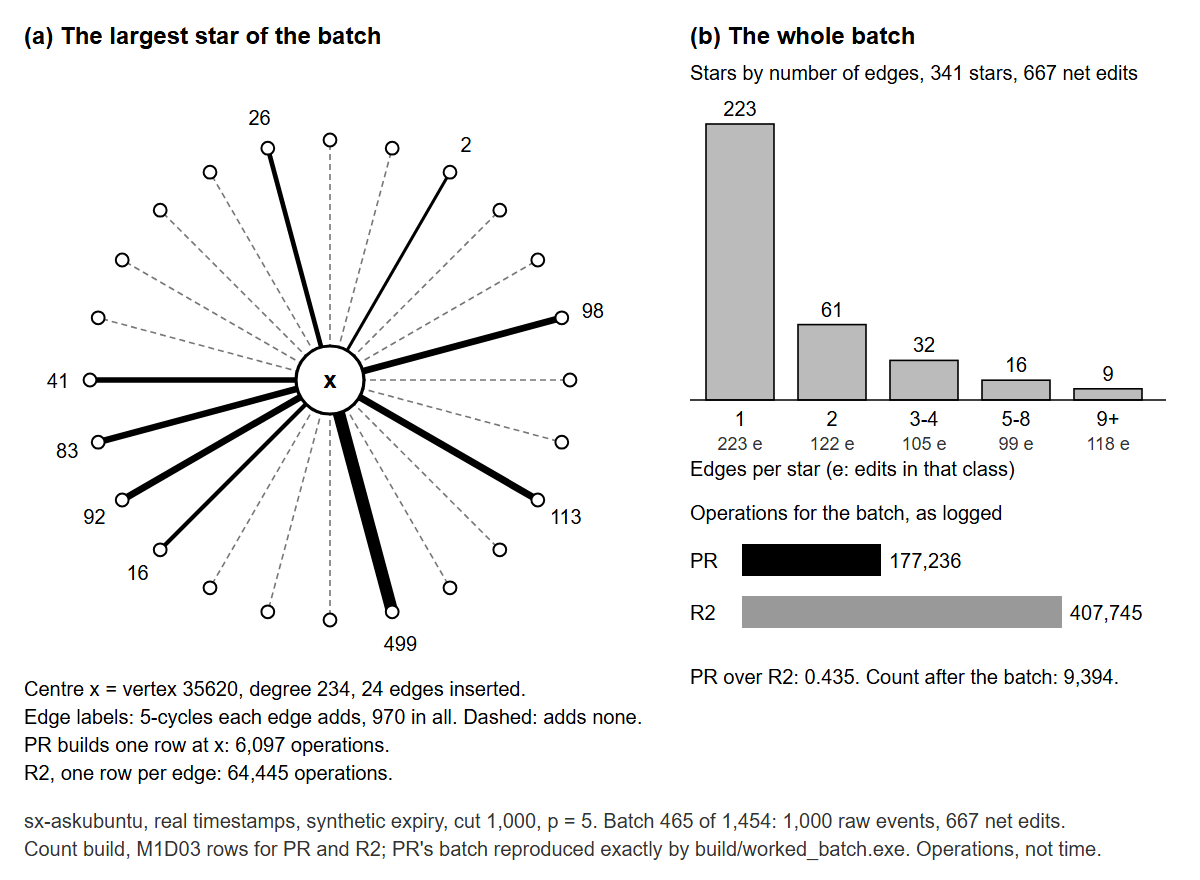
\includegraphics[width=\textwidth]{fig-worked-batch}
  \caption{A worked batch: batch 465 of the 1,454 batches of sx-askubuntu with synthetic expiry, at 1,000 events per batch and $p = 5$. The 1,000 events net to 667 edits. Panel (a) shows the largest star of the batch, 24 insertions at one vertex, each edge labelled with the 5-cycles it adds: PR builds one row at the centre for 6,097 operations, where R2 builds one row per edge for 64,445. Panel (b) shows the whole batch: its 341 stars by number of edges, and the operations of PR and R2, 177,236 against 407,745. The batch was chosen by a rule fixed before any batch was read: the median of PR over R2 among the batches where PR does fewer operations. Operation counts from the count build, not time: on the clock, PR over R2 on this cell is 0.588, a smaller gain than the 0.435 in operations.}
  \label{fig:workedbatch}
\end{figure}
P3 and P4 apply the same idea to triangles and 4-cycles.
They carry a guard that reads only degrees, has no tuned parameter, and whose own operations are counted: a star keeps its row only if the row costs less than the scans it replaces, and otherwise its spokes run as S3 or S4.
The guard is needed because S4 walks from the endpoint of lower degree, while a row is always built at the centre. In early tests, a star at a hub with a few small spokes made P4 slower than S4.
PR has no guard. A guard could only make PR faster, so leaving it out can only understate the gain of sharing.
Reusing one row per vertex across a batch is published for triangle listing by DPTL+~\cite{dptl} and for butterfly counting by BFCB-IG~\cite{bfcb}, and grouping a batch into stars for general patterns by Cheetah~\cite{cheetah}, together with the finding that triangles gain least. We do not claim either.
% gate1.cpp, guards; fivecycle.cpp, FORMS, PR; gate1-protocol.md, Arms; log.md 0019

\paragraph{Wedge Tables.}
T3, T4, WT and WJ keep $W[a, b]$ for every pair of vertices with a common neighbour, and update it on every edge edit.
A delta then becomes a sum of table reads: $W[u, v]$ at $p = 3$, a sum over $N(u)$ at $p = 4$, and at $p = 5$
\[
  \Delta_5(u, v) = \sum_{\substack{a \in N(u),\ c \in N(v) \\ a \neq c}} W[a, c] \;-\; \tau\,(d(u) - 1) \;-\; \tau\,(d(v) - 1),
  \qquad \tau = |N(u) \cap N(v)|,
\]
with $W$ taken in the graph without the pair.
WJ stores the table in one flat hash map.
WT holds the same entries in one open-addressing table per vertex, with each pair stored in both of its tables, so that a join reads only the tables of the shorter list.
Its slots are four bytes, they are searched four at a time with SSE2, and the join switches from probes to one pass over the table against a bitset when that is cheaper.
The layout of WT was chosen by trial on synthetic R-MAT streams~\cite{rmat}, so no stream of this paper shaped it.
T3 and T4 use WT's table.
% fivecycle.cpp, WT and FORMS, WJ; gate1.cpp, T

\paragraph{Mixed Tables.}
M3, M4 and M5 follow the idea of Hanauer, Henzinger and Hua~\cite{hhh}: the table holds only the wedges through light centres, so a hub pays no upkeep, and the wedges through hubs are counted from the adjacency lists at query time.
A vertex turns heavy above degree $2\theta$ and light again below $\theta$, so a switch costs at most $(2\theta)^2$ pairs and is paid for by at least $\theta$ updates.
Writing $H$ for the set of heavy vertices, the hub term at $p = 5$ is $\sum_{h \in H} (A[h] C[h] - T[h])$, with $A[h] = |N(u) \cap N(h)|$, $C[h] = |N(v) \cap N(h)|$ and $T[h] = |N(u) \cap N(v) \cap N(h)|$.
One value of the threshold $\theta$ per pattern was chosen on the engineering streams of Section~\ref{sec:method}, before any evaluation run of a mixed table, from $\{16, 32, \dots, 1024\}$: 16 at $p = 3$ and $p = 4$, and 128 at $p = 5$.
Section~\ref{sec:sensitivity} gives M5 its best $\theta$ per cell instead.
% gate1.cpp, M; gate1-protocol.md, Theta; results/gate1-M1D04/theta.txt; M1D06A

\paragraph{Recount and Published Sharing.}
A4 and A5 recount the cycles inside the ball of radius $r$ around each changed edge, $r = 1$ at $p = 4$ and $r = 2$ at $p = 5$, in the union of the old and new graphs, and take the difference.
The static counters are Chiba and Nishizeki's wedge pairing~\cite{chiba-nishizeki} at $p = 4$ and Algorithm~1 of Shi, Huang and Shun~\cite{shi-huang-shun} at $p = 5$.
B4 ports the batch 4-cycle algorithm BFCB-IG of Wang et al.~\cite{bfcb} from bipartite to general graphs.
It splits a mixed batch into deletions and then insertions, as BFCB-IG does, and builds one row per start vertex that every edit at that vertex reads.
We know of no batch algorithm of this form for 5-cycles, so B4 has no counterpart at $p = 5$.
There is no recount at $p = 3$: in an earlier operation count of ours on six of the streams of Section~\ref{sec:method}, a triangle update cost 5.9 to 13.9 operations, and a recount cannot compete with that.
% gate1.cpp, A and B4; gate1-protocol.md, Arms

\paragraph{Exactness.}
An oracle test compares every arm of every pattern with a brute-force count over vertex tuples, after every batch, on random small graphs whose batches hold deletions, hubs, whole stars, repeated pairs and no-op edits.
Mixed arms run there at $\theta$ down to 1, so vertices switch on graphs this small.
Fourteen mutants, each a plausible way to get an arm wrong, must each fail the test, and so must a naive per-edge sum, which counts a cycle once for each of its changed edges.
On the streams, every arm's count matches every other arm's after every batch, in every timing repeat and in every count build.
% tests/test_gate1.cpp header; CLAUDE.md hard rules 1 and 2; results/gate1-M1D04/README.md

\section{Method of Measurement}
\label{sec:method}

\paragraph{Streams and Their Roles.}
\label{sec:streams}
Twenty streams enter the study, in four sets that were fixed before any of them was timed.
The \emph{engineering} streams, CollegeMsg~\cite{panzarasa-collegemsg}, email-Eu-core-temporal and sx-mathoverflow~\cite{paranjape-motifs}, were used to choose $\theta$ and to fit the cost model of Section~\ref{sec:costmodel}, and never enter a verdict.
The \emph{evaluation} streams, sx-askubuntu, sx-superuser and wiki-talk-temporal~\cite{paranjape-motifs,leskovec-wiki-governance}, decide the first verdict.
These six streams and sx-stackoverflow come from SNAP~\cite{snap}.
The \emph{held-out} stream, sx-stackoverflow, was chosen before any timing run and timed once, at $p = 5$ only.
Hanauer et al.'s set~\cite{hanauer-dyncount} has 56 instances, 18 of them real streams, and four of those 18 are in the first three sets. The \emph{new} streams are 13 of the other 14, chosen by a rule written before their sizes were read: six Wikipedia link streams with real deletions from KONECT, two Reddit hyperlink streams from SNAP~\cite{kumar-reddit}, and five temporal files from Network Repository~\cite{network-repository}.
Each is cut to its first 2,000,000 events, which is Hanauer et al.'s own prefix.
One of them, soc-youtube-growth, has a single timestamp in that prefix and is reported but never scored.
The 38 Kronecker streams of Hanauer et al.'s set are left out as fully synthetic.
Expiry and insert-only variants run on every stream without real deletions, at both batch sizes.
We call one combination of a stream, its variant, a batch size and a pattern size a \emph{cell}.
% gate1-protocol.md, Streams; m1d07-streams.md; docs/figures/fig-test-set.svg; log.md 0025

\paragraph{Operations First.}
Each arm exists in two builds from one source.
The count build counts every unit operation: a list element scanned, a lookup of an edge in the graph's hash map, a row read or write, a table read or write, a degree read, a graph edit, and each step of reducing and grouping the batch.
Operation counts are deterministic and do not depend on the machine, and they were read before any clock.
The timing build has no counters, because a counter in a hot loop is a store the compiler cannot move, and on a synthetic stream the counters cost R2 and PR about 15\% and WJ about 1\%.
All seconds in this paper come from the timing build, and all operation counts from the count build.
Figure~\ref{fig:timeline} shows the count and the operations of five kernels over a whole stream.

\begin{figure}[tbp]
  \centering
  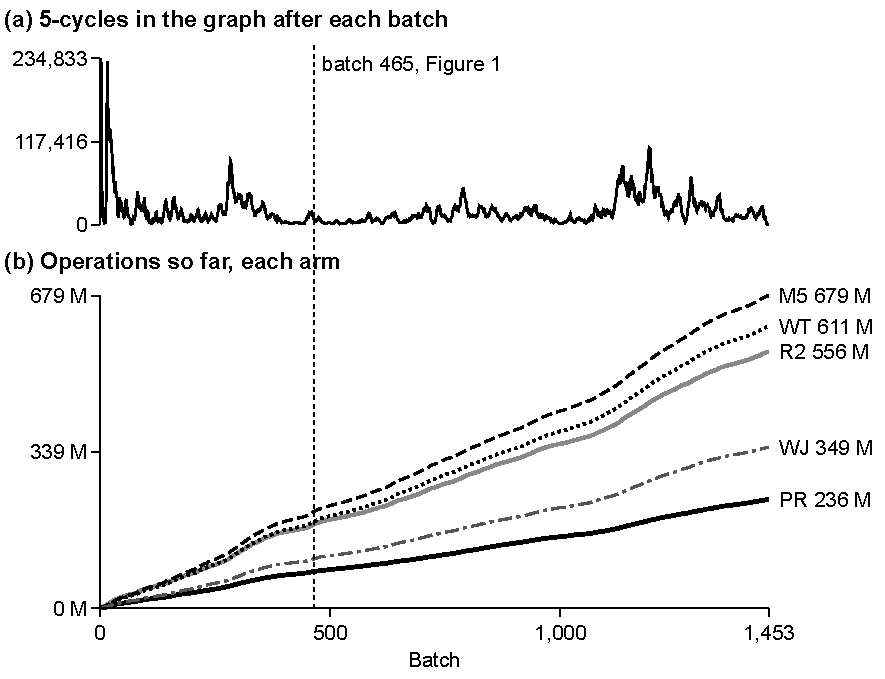
\includegraphics[width=\textwidth]{fig-stream-timeline}
  \caption{The same stream over all 1,454 batches: (a) the 5-cycle count after each batch, and (b) the cumulative operations of PR, R2, WT, WJ and M5. Every kernel's count agrees on every batch. The expiry rule empties the graph by the end of the stream. Operation counts from the count build, not time. On this cell PR also does the fewest operations; on the insert-only cells of the sx streams WJ does fewer operations than PR and is slower, so this cell is not the general case.}
  \label{fig:timeline}
\end{figure}
% fivecycle.cpp header; CLAUDE.md hard rule 3

\paragraph{The Clock.}
All runs are on one machine, an Intel Core Ultra 7 265 with 31\,GB of memory and a 30\,MB last-level cache, under Windows 11, with GCC 16.2 at \texttt{-O2}, linked statically.
One process runs at a time, pinned to one performance core, logical CPU 8.
On a cell whose fastest arm takes under 60\,s each arm runs five times, and otherwise three, with the arms interleaved across repeats in a rotated order.
An arm more than five times slower than the fastest on a cell runs once.
A process stops at 1,200\,s or 16\,GB of committed memory, and A4 and A5 stop at 300\,s.
An arm stopped by time has not finished. It is never counted as a win, and in comparisons its time is its limit.
An arm stopped by memory is out of that cell.
% gate1-protocol.md, Measure; STATUS.md, Environment

\paragraph{The Rule, Fixed Before the Clock.}
Let \emph{share} be P3, P4 or PR, or at $p = 4$ the faster of P4 and B4. Let \emph{best} be the fastest of the other arms, leaving out B4. An arm stopped by its time limit counts in this comparison with its time set to the limit.
A cell \emph{passes} when the slowest repeat of share is at most $0.67$ times the fastest repeat of best.
Comparing the slowest repeat with the fastest is deliberate. In an earlier experiment of ours, a cell passed when the fastest repeats were compared, by a difference of one clock tick, and failed when the slowest of three repeats was used.
A cell's \emph{score} is the ratio of the medians. A cell is \emph{scored} if share and at least one other arm finished or were stopped by time.
The verdict at $p = 5$ is Go if at least a third of the scored cells pass, on at least two streams, with at least two expiry cells among them.
These thresholds, and the treatment of stopped arms, were fixed before the first timing run and were not changed after it.
% gate1-protocol.md, Rule; log.md 0025, reading M1D04-R1

\paragraph{What Exclusive Means.}
The machine is shared with other projects, and timing ran only while it was reserved for this study: no other long or parallel process ran during a timing run.
The machine was not silent.
Scheduled tasks of another project ran every quarter hour, a status mail ran every two hours, and desktop sessions stayed open.
After each timing run, every timed process was checked against the recorded start times of these tasks, and repeats that overlapped one were compared with clean repeats of the same arm on the same cell.
In the last timing run, for the cost model, one of 790 scored repeats overlapped a known task, and it ran 0.2\% over its arm's median.
Section~\ref{sec:sensitivity} gives the same comparison for the runs on the new streams.
% log.md 0025, 0036, 0065; scripts/overlap_check.py; results/cost-M1D10/README.md

\paragraph{Cores.}
To test whether a verdict depends on the core, the 24 cells nearest the pass line were timed again on a performance core and on an efficiency core of the same processor, in one timing run.
The two kinds of core differ in design and in their first two cache levels, and share the last-level cache and memory.
So this is not a second machine, and the paper does not use it as one.
% docs/experiments/m1d08-core-type.md; results/gate1-M1D08/README.md

% Draft 1 of the results, the cost model, the sensitivity analysis and the conclusion, 2026-11-05 (log.md 0067).
% Each paragraph opens with its sentence from writing.md, step 3. The record of each number is in the comment beside it.

\section{Results}
\label{sec:results}

\paragraph{First Verdict.}
On the three evaluation streams, the verdict by the rule fixed before the clock is Go at $p = 5$: 6 of 14 scored cells pass, on all three streams, and 4 of the passes are expiry cells.
At $p = 3$ no cell of 12 passes, and the median score is 1.098, so sharing is slower than the best other kernel there.
At $p = 4$ no cell of 12 passes either, with a median score of 1.299.
The guarded star-row kernel P4 takes 0.094 to 0.323 of the time of the BFCB-IG port on every cell.
% results/gate1-M1D05/README.md

\paragraph{Twelve New Streams.}
On twelve streams that no kernel, parameter or reading of this study had touched before, 22 of 36 scored cells pass at $p = 5$, on 11 of the 12 streams.
Pooled with the first set, 28 of 50 cells pass, on 14 of 16 streams, so the verdict holds on the larger set.
The passes fall under all three labels: 9 of 12 insert-only cells, 6 of 12 expiry cells and 7 of 12 real-deletion cells pass on the new streams, so recorded deletions do not prevent a pass.
Figure~\ref{fig:testset} shows every stream with its label, its size and its passes.
% results/gate1-M1D07T/README.md, readings 1 and 2

\paragraph{Batch Size.}
Passes depend on the batch size.
At batches of 1,000 events, 19 of 25 pooled cells pass, and at batches of 100, 9 of 25 pass.
A larger batch holds more updates at each centre, so the row built once at that centre is reused by more spokes.
Figure~\ref{fig:scorebyp} shows the score of every scored cell against the pattern size, for both batch sizes.
% docs/paper/outline.md claim sentence; pass lists of M1D05 and M1D07T

\paragraph{Where It Fails.}
Two streams give no pass: the held-out stream, sx-stackoverflow, and the Wikipedia stream dewiki.
sx-stackoverflow scores 0.846 and 0.978 on its expiry cells, and on its insert-only cells no kernel finished within the limits, so they are not scored.
dewiki, the largest Wikipedia stream, misses the test at 0.710 and 0.783, with medians of 0.669 and 0.671.
% results/gate1-M1D05/README.md, How much weight; results/gate1-M1D07T/README.md, p = 5 table

\paragraph{Triangles and 4-Cycles.}
At $p = 3$, sharing beats the scan by a median of 13\% on the new streams and never reaches the test.
Pooled over 48 scored cells, the median score at $p = 3$ is 0.965, and the best single cell is 0.700.
So the trend that sharing fails for triangles and pays for larger patterns holds only in its second half: for triangles sharing helps a little, and never by the margin the test asks for.
The new streams have no $p = 4$ cells, and on the first three streams no $p = 4$ cell passes.
% results/gate1-M1D07T/README.md, reading 3

\paragraph{What Sharing Beats.}
The kernel that sharing beats is almost always the scan.
At $p = 5$, R2 is the best other kernel on 43 of 50 pooled cells, and the mixed table M5 or the recount A5 on the other 7.
The wedge tables WT and WJ are the best other kernel on no cell.
So the gain measured here is the gain of the shared row over the same kernel without sharing.
% results/gate1-M1D07T/README.md, Best arm at p = 5

\begin{table}[t]
  \centering
  \begin{tabular}{llrrr}
    \hline
    Set & Label & Scored & Pass & Median score \\
    \hline
    First three streams & insert-only and expiry & 14 & 6 & 0.686 \\
    Twelve new streams & real deletions & 12 & 7 & 0.646 \\
                       & synthetic expiry & 12 & 6 & 0.667 \\
                       & insert-only & 12 & 9 & 0.637 \\
    Pooled & all & 50 & 28 & 0.650 \\
    \hline
  \end{tabular}
  \caption{Cells at $p = 5$. A cell passes when the slowest repeat of PR takes at most 0.67 times the fastest repeat of the best other kernel. The score is the ratio of medians. All streams have real timestamps.}
  \label{tab:p5}
\end{table}
% results/gate1-M1D05/README.md; results/gate1-M1D07T/README.md

\section{Why Operation Counts Mislead: a Cost Model}
\label{sec:costmodel}

\paragraph{Two Winners.}
On 60 of the 76 cells of the newer streams, the kernel with the fewest operations is not the fastest kernel.
On 35 of these cells, at $p = 3$, the scan does the fewest operations and the sharing kernel P3 is fastest.
On 25, at $p = 5$, a wedge table, the mixed table or the recount does the fewest operations and PR is fastest.
The flat wedge table WJ runs at a median of 9.55\,ns per counted operation on these streams, against 0.35\,ns for PR.
% results/gate1-M1D07T/README.md, Operations against the clock

\paragraph{Three Models.}
We fit three linear models of a kernel's median time on a cell to its operation counts on that cell, by nonnegative least squares.
Model U charges one price for every operation.
Model K charges one price for each of ten kinds of operation: a list element scanned, a probe, a row read or write, a degree read, a table read, a table write, a graph edit, a step of netting the batch, a step of grouping it, and a step of a static recount.
Model KC adds an extra price for table probes, reads and writes when the kernel's table is larger than the 30\,MB last-level cache.
The models are fitted on one set of streams and judged on another set that no coefficient has seen, by their median relative error and by how often they name the fastest kernel on a cell.
Kernel-cells under 0.05\,s are left out, since their time is dominated by process start and the clock's resolution.
% docs/experiments/m1d09-cost-model.md; scripts/m1d09_cost.py

\paragraph{Fitted Where Parameters Are Chosen.}
Fitted on the three engineering streams and read on the twelve new streams, model KC names the fastest kernel on 63 of 64 cells, at a median error of 23.0\%.
Model U names 21 of 64, at a median error of 71.3\%.
Fitted instead on the first three evaluation streams, model KC names all 64 at 22.9\%.
Figure~\ref{fig:costmodel} shows predicted against measured time for both fits.
% results/cost-M1D10/README.md; results/cost-M1D09/README.md

\paragraph{The Price of a Probe.}
In both fits a table probe costs about 10 to 18\,ns, and a step along a row or an adjacency list about 0.05 to 0.6\,ns.
The operation counts of different kernels are correlated, so a single coefficient is not a measured price of one instruction.
The ratio between the kinds is stable across the two fits, and it is the reason unit cost fails: the table kernels trade many cheap steps for fewer expensive probes.
% results/cost-M1D10/README.md, Coefficients

\paragraph{No Cache-Size Effect.}
The extra prices for tables larger than the cache add nothing in either fit.
On the new streams, model KC names the same 63 winners as model K, and lowers the median error only from 23.5\% to 23.0\%.
The fit on the first three streams gives the same picture.
So the data do not show that a table outgrowing the last-level cache is what makes the table kernels slow.
% results/cost-M1D10/README.md, Cache; results/cost-M1D09/README.md

\paragraph{What the Model Misses.}
The model does not explain the flat table.
It predicts WJ at a median of 0.15 of its measured time with the engineering fit, and 0.18 with the other.
WJ and the tuned table WT have the same operation counts, and WT runs at 1.42\,ns per operation, so what separates them is not in any counter, table size included.
The engineering fit also fails on the first three streams at $p = 3$ and $p = 4$: there it names the wrong winner on 14 of 24 cells, each time preferring the sharing kernel where the scan is fastest, by margins of 0.3\% to 28\%.
At $p = 5$ it names all 12 correctly.
% results/cost-M1D10/README.md, Read beside it; results/cost-M1D09/README.md

\section{Sensitivity}
\label{sec:sensitivity}

\paragraph{The Mixed Table at Its Best Threshold.}
The mixed table was run on the six first passes at every threshold from 16 to 1,024, and the best threshold on each cell was chosen after the fact.
All six passes hold against it.
The best threshold is 16 on the expiry cells and 64 on the rest, and it beats the scan on one stream only, by 9\%.
Figure~\ref{fig:theta} shows the mixed table's time over the threshold against PR and R2.
% results/gate1-M1D06A/README.md

\paragraph{The Scan Margin.}
Most passes rest on a margin of about 10\% over the scan.
If the best other kernel's fastest repeat were 5\% faster on every cell, 22 of 50 pooled cells would pass, and at 10\% faster 16 of 50, below the third the verdict needs.
A faster scan on another machine could therefore change the verdict, and this is the main reason the result is stated for one machine.
% results/gate1-M1D07T/README.md, How much weight the passes carry

\paragraph{Background Load.}
After each timing run, every timed repeat was checked against the recorded start times of the scheduled tasks on the machine.
In the two timing runs of the new streams, overlapping repeats ran a median of 0.00\% and 0.13\% over their kernel's median on the cell, and clean repeats 0.00\%.
Three passes have every repeat of the best other kernel inside a window, and load can only slow that kernel, so for these passes to be false the load would have had to slow it by 15\% to 57\% in every repeat.
Without the two of these passes whose required slowdown is smallest, and one cell that runs in a few milliseconds, 25 of 47 cells pass.
% results/gate1-M1D07T/README.md, Background load and Robustness

\paragraph{An Efficiency Core.}
The 24 cells nearest the pass line were timed again on a performance core and on an efficiency core of the same processor.
On the performance core, each kernel's median is within 1\% of the earlier run, and the pooled count stays at 28 of 50.
On the efficiency core, 24 of 50 cells pass, and every cell lost is a Wikipedia stream with real deletions.
The efficiency core runs PR and R2 about 1.6 times slower, but not by the same factor on every stream.
% results/gate1-M1D08/README.md

\section{Limits and Conclusion}
\label{sec:conclusion}

\paragraph{One Machine.}
All timing comes from one machine.
The efficiency-core run changes the core and its first two cache levels, and keeps the last-level cache and the memory, so it does not replace a second machine.
Given the scan margin of Section~\ref{sec:sensitivity}, a machine with a relatively faster scan could change the verdict at five vertices.
% results/gate1-M1D08/README.md; docs/experiments/m1d08-core-type.md

\paragraph{Sixteen Streams.}
Sixteen real-timestamp streams are few beside the hundreds of instances in static benchmark sets.
Streams with real timestamps are scarce, and those with recorded deletions more so: they are the real instances of the set of Hanauer et al.~\cite{hanauer-dyncount}, chosen by a rule fixed before their sizes were read, and every one of them is used.
We did not add synthetic streams, because a synthetic stream adds instances without adding evidence about real update patterns.
% docs/experiments/m1d07-streams.md; CLAUDE.md hard rule 4

\paragraph{What Is New.}
The mechanism is not new.
DPTL+ and BFCB-IG reuse a row per vertex across a batch~\cite{dptl,bfcb}, and Cheetah groups batches into stars and reports that triangles gain least~\cite{cheetah}.
What this paper adds is the measured gain of that mechanism against the strongest sequential exact baselines, with every cost inside, on real streams with real deletions and a held-out stream, and a cost model that explains why operation counts choose the wrong kernel.

\paragraph{Conclusion.}
Sharing work inside a batch pays for exact counting of 5-cycles against the strongest sequential baselines we could build, on 28 of 50 cells over 14 of 16 real streams, and it does not pay for triangles or 4-cycles by the same test.
It fails on the held-out stream and on the largest Wikipedia stream, and most passes rest on a margin of about 10\% over the scan.
An engineer choosing among these kernels should price a table probe at about twenty or more times a scan step, rather than count operations, because the operation count chooses the wrong kernel on most cells and the priced model chooses the right one on 63 of 64 unseen cells.


% The figures now sit beside their first mention in the section files (log.md 0068).


\section*{Data and Code Availability}
The source code of every kernel, the scripts that prepare the streams, run the measurements and compute every number in this paper, and the per-cell results are available at \texttt{[repository to be released on acceptance]}.
The input streams are public: SNAP, KONECT and Network Repository, as listed by Hanauer et al.~\cite{hanauer-dyncount}.

\section*{Use of Generative AI}
% Approved by the PI on 2026-11-05 (log.md 0070, bootstrap §9, §21). Drafted from the repository's log and commit history, not from memory.
% The same text, shortened, goes into JGAA's Comments for the Editor field, which JGAA requires.
This study was carried out with an AI assistant, Claude (Anthropic), working under the direction of the corresponding author, who made every decision recorded in the project log.
The assistant was used in four places.
First, it wrote the source code of every kernel, the exactness tests, the stream-preparation scripts and the measurement and analysis scripts.
Second, it wrote the experimental protocols, each committed to version control before the run it governs, and it ran the measurements under those protocols.
Third, it searched and read the literature and drafted the bibliography.
Fourth, it drafted the text of this manuscript and drew its figures.
The output was verified as follows.
Every kernel's count was checked against a brute-force count on random graphs, with deliberately broken versions of each kernel required to fail, and every kernel's count on every batch of every stream was checked against every other kernel's.
Every number in the manuscript was traced to a committed result file.
Every bibliography entry was checked against the publisher's page or the DOI record.
The authors read the full manuscript and approved it as a statement of their own work.
The authors take full responsibility for the content.


\section*{Acknowledgements}
The authors thank Universiti Teknikal Malaysia Melaka (UTeM) for its support.

\bibliographystyle{abbrvurl}
\bibliography{refs}

\clearpage
\appendix
% Every scored cell at p = 5, generated on 2026-11-05 from results/gate1-M1D04/README.md and results/gate1-M1D07T/README.md (log.md 0068).
\section{Every Scored Cell at $p = 5$}
\label{app:cells}
Table~\ref{tab:allcells} lists the 50 scored cells at $p = 5$. The first 14 rows are the three evaluation streams and the held-out stream sx-stackoverflow; the other 36 are the twelve new streams. Seconds are medians of the timing repeats. The score is the ratio of the medians, and the test is the slowest repeat of PR over the fastest repeat of the best other kernel, which passes at 0.67 or less. A best kernel marked $^*$ was stopped at its time limit and enters at that limit.
\begin{table}[p]
\centering
\footnotesize
\setlength{\tabcolsep}{3pt}
\begin{tabular}{llrrlrrrl}
\hline
Stream & Label & Batch & PR s & Best & Best s & Score & Test & Pass \\
\hline
sx-askubuntu & synthetic expiry & 1,000 & 0.268 & R2 & 0.456 & 0.588 & 0.592 & yes \\
sx-askubuntu & synthetic expiry & 100 & 0.429 & R2 & 0.480 & 0.894 & 0.900 & no \\
sx-askubuntu & insert-only & 1,000 & 4.866 & M5 & 11.760 & 0.414 & 0.417 & yes \\
sx-askubuntu & insert-only & 100 & 8.183 & M5 & 11.717 & 0.698 & 0.708 & no \\
sx-superuser & synthetic expiry & 1,000 & 0.469 & R2 & 0.768 & 0.611 & 0.616 & yes \\
sx-superuser & synthetic expiry & 100 & 0.719 & R2 & 0.799 & 0.900 & 0.929 & no \\
sx-superuser & insert-only & 1,000 & 13.254 & R2 & 31.793 & 0.417 & 0.421 & yes \\
sx-superuser & insert-only & 100 & 21.417 & R2 & 31.815 & 0.673 & 0.678 & no \\
wiki-talk-temporal & synthetic expiry & 1,000 & 10.921 & R2 & 36.261 & 0.301 & 0.305 & yes \\
wiki-talk-temporal & synthetic expiry & 100 & 17.519 & R2 & 36.386 & 0.481 & 0.487 & yes \\
wiki-talk-temporal & insert-only & 1,000 & 276.627 & A5$^*$ & 300.000 & 0.922 & 0.955 & no \\
wiki-talk-temporal & insert-only & 100 & 408.891 & A5$^*$ & 300.000 & 1.363 & 1.380 & no \\
sx-stackoverflow & synthetic expiry & 1,000 & 130.920 & R2 & 154.827 & 0.846 & 0.863 & no \\
sx-stackoverflow & synthetic expiry & 100 & 153.099 & R2 & 156.560 & 0.978 & 0.983 & no \\
dewiki & real deletions & 100 & 20.00 & R2 & 29.89 & 0.669 & 0.710 & no \\
dewiki & real deletions & 1,000 & 18.21 & R2 & 27.15 & 0.671 & 0.783 & no \\
frwiki & real deletions & 100 & 33.93 & R2 & 47.74 & 0.711 & 0.725 & no \\
frwiki & real deletions & 1,000 & 29.04 & R2 & 43.84 & 0.662 & 0.665 & yes \\
itwiki & real deletions & 100 & 47.97 & R2 & 103.82 & 0.462 & 0.482 & yes \\
itwiki & real deletions & 1,000 & 38.12 & R2 & 96.73 & 0.394 & 0.426 & yes \\
nlwiki & real deletions & 100 & 30.49 & R2 & 44.36 & 0.687 & 0.692 & no \\
nlwiki & real deletions & 1,000 & 25.37 & R2 & 39.57 & 0.641 & 0.643 & yes \\
plwiki & real deletions & 100 & 41.10 & R2 & 63.23 & 0.650 & 0.670 & no \\
plwiki & real deletions & 1,000 & 35.21 & R2 & 59.16 & 0.595 & 0.596 & yes \\
simplewiki & real deletions & 100 & 14.14 & R2 & 24.36 & 0.581 & 0.591 & yes \\
simplewiki & real deletions & 1,000 & 9.99 & R2 & 17.24 & 0.580 & 0.614 & yes \\
ia-enron-email-dynamic & synthetic expiry & 100 & 0.55 & R2 & 0.97 & 0.568 & 0.577 & yes \\
ia-enron-email-dynamic & synthetic expiry & 1,000 & 0.47 & R2 & 0.89 & 0.527 & 0.533 & yes \\
ia-enron-email-dynamic & insert-only & 100 & 1.26 & R2 & 2.23 & 0.567 & 0.571 & yes \\
ia-enron-email-dynamic & insert-only & 1,000 & 1.16 & R2 & 2.22 & 0.523 & 0.531 & yes \\
ia-reality-call & synthetic expiry & 100 & 0.01 & R2 & 0.01 & 1.000 & 1.000 & no \\
ia-reality-call & synthetic expiry & 1,000 & 0.00 & R2 & 0.01 & 0.800 & 0.800 & no \\
ia-reality-call & insert-only & 100 & 0.00 & R2 & 0.00 & 1.000 & 1.000 & no \\
ia-reality-call & insert-only & 1,000 & 0.00 & R2 & 0.00 & 0.667 & 0.667 & yes \\
soc-redditHyperlinks-body & synthetic expiry & 100 & 0.14 & R2 & 0.15 & 0.934 & 0.940 & no \\
soc-redditHyperlinks-body & synthetic expiry & 1,000 & 0.09 & R2 & 0.14 & 0.686 & 0.691 & no \\
soc-redditHyperlinks-body & insert-only & 100 & 0.98 & R2 & 1.10 & 0.888 & 0.889 & no \\
soc-redditHyperlinks-body & insert-only & 1,000 & 0.68 & R2 & 1.10 & 0.618 & 0.625 & yes \\
soc-redditHyperlinks-title & synthetic expiry & 100 & 0.73 & R2 & 0.83 & 0.884 & 0.889 & no \\
soc-redditHyperlinks-title & synthetic expiry & 1,000 & 0.41 & R2 & 0.77 & 0.539 & 0.544 & yes \\
soc-redditHyperlinks-title & insert-only & 100 & 5.22 & R2 & 5.77 & 0.904 & 0.905 & no \\
soc-redditHyperlinks-title & insert-only & 1,000 & 3.59 & R2 & 5.77 & 0.622 & 0.633 & yes \\
soc-wiki-elec & synthetic expiry & 100 & 0.12 & R2 & 0.20 & 0.624 & 0.628 & yes \\
soc-wiki-elec & synthetic expiry & 1,000 & 0.08 & A5 & 0.10 & 0.827 & 0.845 & no \\
soc-wiki-elec & insert-only & 100 & 0.55 & R2 & 0.84 & 0.657 & 0.657 & yes \\
soc-wiki-elec & insert-only & 1,000 & 0.51 & R2 & 0.83 & 0.611 & 0.614 & yes \\
tech-as-topology & synthetic expiry & 100 & 1.51 & R2 & 2.33 & 0.647 & 0.649 & yes \\
tech-as-topology & synthetic expiry & 1,000 & 0.90 & R2 & 2.33 & 0.384 & 0.385 & yes \\
tech-as-topology & insert-only & 100 & 0.86 & M5 & 1.32 & 0.651 & 0.657 & yes \\
tech-as-topology & insert-only & 1,000 & 0.53 & M5 & 1.33 & 0.397 & 0.400 & yes \\
\hline
\end{tabular}
\caption{The 50 scored cells at $p = 5$, 28 of which pass. All streams have real timestamps.}
\label{tab:allcells}
\end{table}


\end{document}
